\documentclass[9pt]{beamer} 

\pdfoutput=1 

\makeatletter 

%----------------------------------------------------------------------------%

\usepackage{amscd}
\usepackage{amsmath}
\usepackage{amsthm}
\usepackage{amsxtra}
\usepackage[english]{babel} 
\usepackage{color}
\usepackage[T1]{fontenc} 
\usepackage{geometry} 
\usepackage{hyperref} 
\usepackage[utf8]{inputenc} 
\usepackage{lmodern}
\usepackage{manfnt}
\usepackage[numbers,sort]{natbib}
\usepackage{tikz}
\usepackage{url}
\usepackage{xcolor}

%----------------------------------------------------------------------------%

\beamertemplatenavigationsymbolsempty

\setbeamertemplate{footline}[frame number]

\setbeamersize{text margin left=20pt,text margin right=20pt}

\setbeamercolor{title page}{bg=white!96!black,fg=red!44!black}
\setbeamercolor{frametitle}{bg=white,fg=red!44!black}
\setbeamercolor{normal text}{black}
\setbeamercolor{block title}{bg=black!20!white,fg=red!44!black}
\setbeamercolor{block body}{bg=black!20!white,fg=black}
\setbeamercolor{block title example}{bg=black!10!white,fg=red!44!black}
\setbeamercolor{block body example}{bg=black!10!white,fg=black}
\setbeamercolor{enumerate item}{bg=white!96!black,fg=red!44!black}
\setbeamercolor{enumerate subitem}{bg=white!96!black,fg=red!44!black}
\setbeamercolor{enumerate subsubitem}{bg=white!96!black,fg=red!44!black}
\setbeamercolor{itemize item}{bg=white!96!black,fg=red!44!black}
\setbeamercolor{itemize subitem}{bg=white!96!black,fg=red!44!black}
\setbeamercolor{itemize subsubitem}{bg=white!96!black,fg=red!44!black}

\setbeamerfont{title}{size={\LARGE},series={\bf}}
\setbeamerfont{author}{size={\Large},series={\bf}}
\setbeamerfont{institute}{size={\normalsize},series={\tt}}
\setbeamerfont{conference}{size={\large},series={\tt}}
\setbeamerfont{date}{size={\normalsize},series={\tt}}
\setbeamerfont{coauthor}{size={\normalsize},series={\bf}}
\setbeamerfont{paper}{size={\normalsize},series={\tt}}
\setbeamerfont{frametitle}{size={\normalsize},series={\bf}}
\setbeamerfont{block title}{size={},series={}}
\setbeamerfont{block body}{size={},series={}}
\setbeamerfont{block title example}{size={},series={}}
\setbeamerfont{block body example}{size={},series={}}

\newcommand\coauthor[1]{\def\insertcoauthor{#1}}
\coauthor{}

\newcommand\conference[1]{\def\insertconference{#1}}
\conference{}

\newcommand\paper[1]{\def\insertpaper{#1}}
\paper{}

\defbeamertemplate*{title page}{sobre}[1][]
{%
\vfill
{\usebeamerfont{title}\inserttitle}\\
\vspace*{22pt}
{\usebeamerfont{author}\color{black}\insertauthor}\\
\vspace*{8pt}
{\usebeamerfont{institute}\color{black}\insertinstitute}\\
\vspace*{8pt}
{\usebeamerfont{conference}\color{black}\insertconference}\\
\vspace*{8pt}
{\usebeamerfont{date}\color{black}\insertdate}\\
\vspace*{22pt}
{\usebeamerfont{coauthor}\color{black} joint work with \insertcoauthor}\\
\vspace*{8pt}
{\usebeamerfont{paper}\color{black}\insertpaper}
\vfill
}%  

\newcommand{\sm}[1]{\left\langle#1\right\rangle}

%----------------------------------------------------------------------------%

\hypersetup{     
unicode=false,      
pdftoolbar=true,    
pdfmenubar=true,    
pdffitwindow=true,  
pdfstartview={FitH},
pdftitle={lpt-seminar-antoine},    
pdfauthor={Antoine Géré},     
pdfsubject={Mathematical Physics},   
pdfcreator={LaTeX},  
pdfproducer={pdfTex},
pdfkeywords={Non-Commutative Geometry, Differential and Algebraic Geometry, Matrix Models, Models of Quantum Gravity},  
pdfnewwindow=true,  
citecolor=darkcerulean,
}

%----------------------------------------------------------------------------%

\title{Perturbatively finite gauge models on the noncommutative three-dimensional space \texorpdfstring{$\mathbb{R}^3_\lambda$}{R3l}}

\author{Antoine Géré}

\institute{Università degli studi di Genova, Dipartimento di Matematica}

\conference{Seminar in Mathematical Physics -- LPT Orsay}

\date{May 26th, 2016}

\coauthor{Tajron Jurić and Jean-Christophe Wallet}

\paper{JHEP \textbf{12} (2015) 045, [arxiv:1507.08086]}

%============================================================================%
\begin{document}
%============================================================================%

\selectlanguage{english}

%----------------------------------------------------------------------------%

\begin{frame}[plain]
\titlepage
\end{frame}

%----------------------------------------------------------------------------%

\begin{frame}

\frametitle{Plan}

{\Large{
\begin{itemize}

\item \textbf{Noncommutative space $\mathbb{R}^3_\lambda$} \\[30pt]

\item \textbf{Family of gauge invariant action} \\[30pt]

\item \textbf{Finiteness to all orders} \\[30pt]

\item \textbf{Link to exactly solvable models}

\end{itemize}
}}

\end{frame}

%----------------------------------------------------------------------------%

\begin{frame}

\frametitle{Noncommutative space $\mathbb{R}^3_\lambda$}

\vspace*{-10pt}

\begin{equation*}
\tikz[baseline]{\node[fill=black!28!white,anchor=base] (t1) {$\mathbb{R}^3_\lambda = \mathbb{C}\left[x_1,x_2,x_3,x_0\right] \setminus \mathcal{I}\left[\mathcal{R}_1,\mathcal{R}_2\right]$
}
;}
\end{equation*}

$\bullet$ $\mathbb{C}\left[x_1,x_2,x_3,x_0\right]$ : free algebra generated by coordinates $x_1, x_2, x_3$ and $x_0$

\vspace*{8pt}

$\bullet$ $\mathcal{I}\left[\mathcal{R}_1,\mathcal{R}_2\right]$ : two sided ideal generated by the relations
\vspace*{-5pt}
\begin{equation*}
\mathcal{R}_1 : \left[x_\mu,x_\nu\right] = i \lambda \epsilon_{\mu\nu\rho} x_\rho \qquad
\mathcal{R}_2 : x_0^2 + \lambda x_0 = \sum_{\mu=1}^{3} x_\mu^2
\vspace*{-5pt}
\end{equation*}

\quad $\to$ \ unital $\ast$ algebra (involution : complex conjugation)

\vspace*{4pt}

\quad $\to$ \ center $\mathcal{Z}\left(\mathbb{R}^3_\lambda\right)$ generated by $x_0$

\vspace*{8pt}

\textbf{Element on $\mathbb{R}^3_\lambda = \left(
\underset{j\in\frac{\mathbb{N}}{2}}{\bigoplus} \ \mathbb{M}_{2j+1}\left(\mathbb{C}\right), \cdot\right)$}

\vspace*{1pt}

\begin{equation*}
\phi = \sum_{j\in\frac{\mathbb{N}}{2}} \sum_{-j \leq m, n \leq j} \phi^j_{mn} \ 
\tikz[baseline]{\node[fill=black!28!white,anchor=base] (t1) {$v^j_{mn}$};} \hspace*{2pt} \leadsto \hspace*{2pt} \mbox{orthogonal basis :} \ \left\{ v^j_{mn} , j\in\frac{\mathbb{N}}{2} , -j \leq m,n \leq j \right\} 
\vspace*{-5pt}
\end{equation*}

\vspace*{8pt}

\textbf{Scalar product} \ $\sm{\phi , \psi} = \mbox{Tr}\left( \phi^\dagger \psi \right)$

\begin{eqnarray*}
\mbox{Tr}\left( \phi \psi \right) = 8 \pi \lambda^3 \sum_{j\in\frac{\mathbb{N}}{2}} w(j) \ \mbox{tr}_j\left(\phi^j \ \psi^j\right) = 8 \pi \lambda^3 \sum_{j\in\frac{\mathbb{N}}{2}} w(j) \sum_{-j \leq m, n \leq j} \phi^j_{mn} \ \psi^j_{mn}
\vspace*{-5pt}
\end{eqnarray*}

\vfill

\end{frame}

%----------------------------------------------------------------------------%

\begin{frame}

\frametitle{Differential calculus}

\vfill

$\bullet$ Lie algebra of real inner derivation
\vspace*{-2pt}
\begin{eqnarray*}
&& \mathcal{G} = \left\{ D_\mu \cdot = i \left[ \theta_\mu , \cdot \right] \ , \quad \theta_\mu = \frac{x_\mu}{\lambda^2} \right\} \\
&& \mbox{with } \ \left[ D_\mu , D_\nu \right] = - \frac{1}{\lambda} \epsilon_{\mu\nu\rho} D_\rho  , \quad \forall \mu, \nu, \rho = 1, 2, 3 
\vspace*{-2pt}
\end{eqnarray*}

\vfill

$\bullet$ \textbf{Connection} on right module $\mathbb{M}$ over $\mathbb{R}^3_\lambda$ \ : \quad \tikz[baseline]{\node[fill=black!28!white,anchor=base] (t1) {$\nabla : \mathcal{G} \times \mathbb{M} \to \mathbb{M}$};}\\[2pt]
\quad \textdbend \quad $\leadsto$ \quad particular choice : $\mathbb{M} = \mathbb{R}^3_\lambda$
\vspace*{-2pt}
\begin{eqnarray*}
\nabla_{D_\mu}(a) :=  \nabla_\mu(a) = D_\mu a + A_\mu a \ , \ \ 
\tikz[baseline]{\node[fill=black!28!white,anchor=base] (t1) {$A_\mu = \nabla_\mu(\mathbb{I})$};}
 \ , \ \
\tikz[baseline]{\node[fill=black!28!white,anchor=base] (t1) {$A_\mu^\dagger = - A_\mu$};}
\vspace*{-2pt}
\end{eqnarray*}

\vfill

$\bullet$ \textbf{Curvature}
\vspace*{-2pt}
\begin{eqnarray*}
&& F(X,Y) = \left[\nabla_X , \nabla_Y\right] - \nabla_{[X,Y]} \\[2pt]
&& F(D_\mu,D_\nu) := \tikz[baseline]{\node[fill=black!28!white,anchor=base] (t1) {$F_{\mu\nu} = D_\mu A_\nu - D_\nu A_\mu + \left[A_\mu , A_\nu\right] + \frac{1}{\lambda} \epsilon_{\mu\nu\rho} A_\rho$};}
\end{eqnarray*}

\vfill

\end{frame}

%----------------------------------------------------------------------------%

\begin{frame}

\frametitle{Gauge transformation}

$\bullet$ \ group of \textbf{unitary elements} \ $\mathcal{U}\left(\mathbb{R}^3_\lambda\right)$ with \textbf{left action}

\qquad $\to$ for any $\phi\in\mathbb{R}^3_\lambda$ and $g\in\mathcal{U}\left(\mathbb{R}^3_\lambda\right)$

\begin{equation*}
g^\dagger g = 1 \ , \quad \phi^g = g \phi \ , \quad \nabla_\mu^g = g^\dagger \nabla_\mu \circ g
\end{equation*}

thus
\vspace*{-1pt}
\begin{equation*}
\tikz[baseline]{\node[fill=black!28!white,anchor=base] (t1) {$A_\mu^g = g^\dagger A_\mu \ g + g^\dagger D_\mu \ g \ , \ \ \mbox{and } \quad F^g_{\mu\nu} = g^\dagger F_{\mu\nu} \ g$};}
\end{equation*}
\vspace*{1pt}

$\bullet$ \ $\exists$ \textbf{gauge invariant connection} and \textbf{curvature}

\begin{equation*} 
\nabla^{inv}_\mu(a) = D_\mu a - i \theta_\mu a = - i a \theta_\mu \quad \mbox{and} \quad F^{inv}_{\mu\nu}=0
\end{equation*}

$\bullet$ \ \textbf{Covariant coordinates}

\begin{equation*}
\nabla_\mu - \nabla^{inv}_\mu := \tikz[baseline]{\node[fill=black!28!white,anchor=base] (t1) {$\mathcal{A}_\mu = A_\mu + i \theta_\mu$};} \quad \mbox{and} \quad \tikz[baseline]{\node[fill=black!28!white,anchor=base] (t1) {$\mathcal{A}_\mu^\dag = - \mathcal{A}_\mu$};}
\end{equation*}
then
\vspace*{-2pt}
\begin{equation*} 
F_{\mu\nu} = \left[\mathcal{A}_\mu,\mathcal{A}_\nu\right] + \frac{1}{\lambda} \epsilon_{\mu\nu\rho} \mathcal{A}_\rho
\end{equation*}

\end{frame}

%----------------------------------------------------------------------------%

\begin{frame}

\frametitle{Family of gauge invariant classical action I}

Convenient to work with hermitean fields

\begin{equation*}
\mathcal{A}_\mu = i \Phi_\mu \quad \leadsto \quad \Phi_\mu^\dag = \Phi_\mu
\end{equation*}

\textbf{gauge-invariant} functional (classical) \textbf{actions} \\
$\to$ \textbf{trace} of \textbf{gauge-covariant polynomial} in the covariant coordinates
%
\begin{equation*}
S_{inv}(\Phi_\mu) = \mbox{Tr}\left(P(\Phi_\mu)\right) 
\end{equation*}

Natural requirement for the gauge-invariant functional are:

\begin{enumerate}
\item $P(\Phi_\mu)$ is \textbf{at most quartic} in $\Phi_\mu$,
\item $P(\Phi_\mu)$ \textbf{does not involve linear term} in $\Phi_\mu$ \\
$\to$ \ (no tadpole at the classical order)
\item the \textbf{kinetic operator} is \textbf{positive}
\end{enumerate}

\vspace*{10pt}

$\leadsto$ \ \textbf{gauge-invariant harmonic term} $\sim\mbox{Tr}(x^2\Phi_\mu \Phi_\mu)$
\vspace*{-2pt}
\begin{equation*}
x^2 := \sum_{\mu=1}^3x_\mu x_\mu \in \mathcal{Z}(\mathbb{R}^3_\lambda)
\end{equation*}

\end{frame}

%----------------------------------------------------------------------------%

\begin{frame}

\frametitle{Family of gauge invariant classical action II}

\vfill

\textbf{Requirements \textcolor{black}{1} and \textcolor{black}{2} give :}
\vspace*{-2pt}
\begin{eqnarray*}
S(\Phi) &=& 
\frac{1}{g^2} \mbox{Tr}\left( 2(\Omega+1) \Phi_\mu \Phi_\nu \Phi_\nu \Phi_\mu + 2(\Omega-1) \Phi_\mu \Phi_\nu \Phi_\mu \Phi_\nu \right.\\
&& \qquad \left. + i \zeta \epsilon_{\mu\nu\rho} \Phi_\mu \Phi_\nu \Phi_\rho + (M+\mu x^2) \Phi_\mu \Phi_\mu \right)
\end{eqnarray*}

$S(\Phi)$ is positive when 
\vspace*{-2pt}
\begin{equation*}
\tikz[baseline]{\node[fill=black!28!white,anchor=base] (t1) {$\Omega\geq0,\ \mu>0,\ \zeta=0,\ M>0$};}
\quad\mbox{or}\quad
\tikz[baseline]{\node[fill=black!28!white,anchor=base] (t1) {$\Omega\geq0,\ \mu>0,\ \zeta=\frac{4}{\lambda},\ M>\frac{2}{\lambda^2}$};}
\end{equation*}

thus
\vspace*{-2pt}
\begin{equation*}
S_\Omega = \frac{1}{g^2} \mbox{Tr}\big((F_{\mu\nu} - \frac{i}{\lambda} \epsilon_{\mu\nu\rho} \Phi_\rho)^\dag (F_{\mu\nu} - \frac{i}{\lambda} \epsilon_{\mu\nu\rho} \Phi_\rho) + \Omega\left\{\Phi_\mu,\Phi_\nu\right\}^2 + (M+\mu x^2) \Phi_\mu \Phi_\mu \big)
\end{equation*}

\vfill

\textbf{Equation of motion}
\vspace*{-2pt}
\begin{equation*}
4(\Omega+1)(\Phi_\rho\Phi_\mu\Phi_\mu+\Phi_\mu\Phi_\mu\Phi_\rho)+8(\Omega-1)\Phi_\mu\Phi_\rho\Phi_\mu+2(M+\mu x^2) \Phi_\rho = 0
\end{equation*}

\tikz[baseline]{\node[fill=black!28!white,anchor=base] (t1) {
$\Phi_\rho=0$ is the absolute minimum
};}

\vfill

\end{frame}

%----------------------------------------------------------------------------%

\begin{frame}

\frametitle{Kinetic operator of the classical action}

\vfill

We have

\begin{equation*}
\tikz[baseline]{\node[fill=black!28!white,anchor=base] (t1) {$S_\Omega(\Phi) = S_{Kin}(\Phi) + \frac{1}{g^2} \mbox{Tr}\left((F_{\mu\nu} - \frac{i}{\lambda} \epsilon_{\mu\nu\rho} \Phi_\rho)^\dag (F_{\mu\nu} - \frac{i}{\lambda} \epsilon_{\mu\nu\rho} \Phi_\rho) + \Omega\left\{\Phi_\mu,\Phi_\nu\right\}^2\right)
$};}
\end{equation*}

\vspace*{14pt}

\textbf{Kinetic term} of the classical action $S_\Omega$ :

\begin{eqnarray*}
S_{Kin}(\Phi) &=& \frac{1}{g^2} \mbox{Tr}\left( \Phi_\mu (M+\mu x^2) \Phi_\mu\right) \\
&=& \frac{1}{g^2} \mbox{Tr}\left( \Phi_\mu G \Phi_\mu\right)
\end{eqnarray*}

\vspace*{12pt}

with the \textbf{positive self-adjoint operator} written in the basis

\begin{equation*}
\tikz[baseline]{\node[fill=black!28!white,anchor=base] (t1) {$G^{j_1j_2}_{mn;kl} = \frac{8\pi\lambda^3}{g^2} w(j_1) \ \left(M+\lambda^2\mu j_1(j_1+1)\right) \delta^{j_1j_2} \delta_{nk} \delta_{ml}$};}
\end{equation*}


\vfill

\end{frame}

%----------------------------------------------------------------------------%

\begin{frame}

\frametitle{Gauge fixing I}

\vfill

$\bullet$ \ \textbf{BRST operation} $\delta_0$

\begin{equation*}
\delta_0 \Phi_\mu = i [C,\Phi_\mu]
\end{equation*}

\begin{itemize}
\item $C$ : the ghost field

\item $\delta_0$ acts as antiderivation w.r.t. grading
\end{itemize}

\vfill

$\bullet$ \ \textbf{Fixing the gauge symmetry :}

\begin{equation*}
\Phi_3=\theta_3 \quad \mbox{thus} \quad \delta_0 {\bar{C}} = b \quad \delta_0b = 0
\end{equation*}

\begin{itemize}
\item where ${\bar{C}}$ : the antighost field
\item and $b$ : the St\"uckelberg field
\end{itemize}

\vfill

$\bullet$ \ \textbf{BRST invariant gauge-fixing term}

\begin{equation*}
S_{fix}=\delta_0\mbox{Tr}\big({\bar{C}}(\Phi_3-\theta_3) \big)=\mbox{Tr}\big(b(\Phi_3-\theta_3)-i{\bar{C}}[C,\Phi_3]\big)
\end{equation*}

Integration over the St\"ueckelberg field $b$ \ $\to$ \ constraint $\Phi_3=\theta_3$

\vfill

\end{frame}

%----------------------------------------------------------------------------%

\begin{frame}

\frametitle{Gauge fixing II}

\vfill

$\bullet$ \ \textbf{Gauge-fixed action}

\begin{equation*}
S^f_\Omega=S_2+S_4
\end{equation*}

with
\vspace*{-2pt}
\begin{eqnarray*}
S_4 &=& \frac{4}{g^2} \mbox{Tr} \left( \Omega (\Phi_1^2 + \Phi_2^2)^2 + (\Omega-1)(\Phi_1\Phi_2\Phi_1\Phi_2 - \Phi_1^2\Phi_2^2) \right) \\
S_2 &=& \frac{1}{g^2} \mbox{Tr} \left((\Phi_1,\Phi_2)
\begin{pmatrix}
Q&0\\
0&Q
\end{pmatrix} 
\begin{pmatrix}
\Phi_1\\
\Phi_2
\end{pmatrix} 
\right) \\[2pt]
Q &=& G+8\Omega L(\theta_3^2) + i4 (\Omega-1) L(\theta_3) D_3 
\end{eqnarray*}

where $G=M+\mu x^2$ and $L(X)$ is the left multiplication by $X$.\\[4pt]

\vfill

$\bullet$ \ \textbf{Particular case :} $\Omega=1$

\begin{itemize}
\item Kinetic operator : $K = G+8\Omega L(\theta_3^2)$ 
\item Interaction term : $S_4 = \frac{4}{g^2} \mbox{Tr} \left( \left(\Phi_1^2 + \Phi_2^2\right)^2\right)$
\end{itemize}
\end{frame}

%----------------------------------------------------------------------------%

\begin{frame}

\frametitle{Gauge-fixed action at $\Omega=1$}

\vfill

\vspace*{-5pt}
\begin{equation*}
S^f_{\Omega=1} = \frac{1}{g^2} \mbox{Tr}\left( (\Phi_1,\Phi_2)
\begin{pmatrix}
K&0\\
0&K
\end{pmatrix} 
\begin{pmatrix}
\Phi_1\\
\Phi_2
\end{pmatrix} 
\right)
+ \frac{4}{g^2} \mbox{Tr}\left( \left(\Phi_1^2 + \Phi_2^2\right)^2\right)
\end{equation*}

\vspace*{10pt}

\textbf{Kinetic operator}

\begin{eqnarray*}
&& K = G+8\Omega L(\theta_3^2) \\
&& K^{j_1 j_2}_{mn;kl} = \frac{8\pi\lambda^3}{g^2} w(j_1) \left( M + \mu \lambda^2 j_1 (j_1+1) + \frac{4}{\lambda^2} (k^2+l^2) \right) \delta^{j_1j_2} \delta_{ml} \delta_{nk}
\end{eqnarray*}

It verifies
%
\begin{equation*}
K^{j_1j_2}_{mn;kl} = K^{j_1j_2}_{lk;nm} = K^{j_1j_2}_{mn;lk} 
\end{equation*}
%
reflecting reality of the functional action and the self-adjointness of $K$.

\vspace*{10pt}

\textbf{Inverse of $K$}
%
\begin{equation*}
\sum_{j_2,k,l} K^{j_1j_2}_{mn;lk} P^{j_2j_3}_{kl;rs} = \delta^{j_1j_3} \delta_{ms} \delta_{nr} \qquad \sum_{j_2,n,m} P^{j_1j_2}_{rs;mn} K^{j_2j_3}_{nm;kl} = \delta_{j_1j_3} \delta_{rl} \delta_{sk}
\end{equation*}
%
\begin{equation*}
\leadsto \quad P^{j_1j_2}_{mn;kl} = \frac{g^2}{8\pi\lambda^3} \frac{1}{w(j_1)(M+\lambda^2\mu j_1(j_1+1)+\frac{4}{\lambda^2}(k^2+l^2))}\delta^{j_1j_2}\delta_{ml}\delta_{nk}
\end{equation*}

\vfill

\end{frame}

%----------------------------------------------------------------------------%

\begin{frame}

\frametitle{One loop 2-point function}

Contribution to the quadratic part at one-loop

\begin{equation*}
\Gamma^1_2(\Phi_\alpha)=\frac{32\pi\lambda^3}{g^2}\sum_{-j\le m,n,r,p\le j}(\phi_\alpha)^j_{mn}\left( \sigma^{NP\ j}_{pr;mn} + \sigma^{P\ j}_{pr;nm} \right)(\phi_\alpha)^j_{kl} 
\end{equation*}

with

\begin{eqnarray*}
\sigma^{NP\ j}_{pr;mn} &=& w(j)P^j_{pr;mn} \ \sim \ \frac{1}{(M+\lambda^2\mu j(j+1)+\frac{4}{\lambda^2}(m^2+n^2))} \\
%
\sigma^{P\ j}_{pr;nm} &=& 3\delta_{mp}\sum_{m=-j}^jw(j)P^j_{rm;mn} 
\ \sim \ \sum_{m=-j}^j \frac{1}{(M+\lambda^2\mu j(j+1)+\frac{4}{\lambda^2}(m^2+n^2))}
\end{eqnarray*}

\begin{itemize}
\item $\sigma^{NP}$ is finite for $j=0$ and $j\to\infty$

\item $\sigma^{P}$ is also finite for $j=0$ and $j\to\infty$
%
\begin{eqnarray*}
\sum_{m=-j}^j w(j)P_{rm;mn} &\leq& \frac{2j+1}{\left(M+\lambda^2\mu j(j+1)\right)}
\end{eqnarray*}
\end{itemize}


\end{frame}

%----------------------------------------------------------------------------%

\begin{frame}

\frametitle{One loop 4-point function}

Typical planar contributions 

\begin{eqnarray*}
\Gamma^{P\ 1}_4 \sim \sum\left(\sum_{-j\le p,q\le j}w^2(j)P^j_{n_1p;qr_2}P^j_{pm_2;s_1q}\delta_{m_1n_2}\right) \ \delta_{s_2r_1} (\phi_\alpha)^j_{m_1m_2}(\phi_\alpha)^j_{n_1n_2}(\phi_\alpha)^j_{r_1r_2}(\phi_\alpha)^j_{s_1s_2}
\end{eqnarray*}

finite for any value of $j$ and decays to $0$ when $j\to\infty$ due to the estimate :

\begin{equation*}
\sum_{-j\le p,q\le j}w^2(j)P^j_{n_1p;qr_2}P^j_{pm_2;s_1q}\le\delta_{n_1r_2}
\delta_{s_1m_2} \frac{(2j+1)}{(M+\lambda^2\mu j(j+1))^2}
\end{equation*}

Three species of non-planar contributions 

\begin{eqnarray*}
&& \Gamma^1_{14}\sim\sum \left(w^2(j) P^j_{m_1n_2;s_1r_2} P^j_{n_1m_2;r_1s_2}\right)(\phi_\alpha)^j_{m_1m_2}(\phi_\alpha)^j_{n_1n_2}(\phi_\alpha)^j_{r_1r_2}(\phi_\alpha)^j_{s_1s_2}\\
%
&& \Gamma^1_{24} \sim \sum \left( \sum_p w^2(j) P^j_{m_1p;s_1r_2} P^j_{pn_2;r_1s_2} \delta_{m_2n_1} \right) \ (\phi_\alpha)^j_{m_1m_2}(\phi_\alpha)^j_{n_1n_2}(\phi_\alpha)^j_{r_1r_2}(\phi_\alpha)^j_{s_1s_2}\\
&& \Gamma^1_{34}\sim\sum\left(\sum_{p,q}w^2(j)P^j_{pm_2;qs_2}P^j_{n_1p;s_1q}
\delta_{m_1n_2}\delta_{s_2r_1} \right) \ (\phi_\alpha)^j_{m_1m_2}(\phi_\alpha)^j_{n_1n_2}(\phi_\alpha)^j_{r_1r_2}(\phi_\alpha)^j_{s_1s_2}
\end{eqnarray*}

possible to find estimates to show this contribution are also finite for any value of $j$

\end{frame}

%----------------------------------------------------------------------------%

\begin{frame}

\frametitle{Finiteness -- ``Truncated model'' I}

\begin{itemize}
\item gauge choice : $\Phi_3 = 0$

\item propagator of the truncated theory : 

\begin{equation*}
(G^{-1})^{j_1j_2}_{mn;kl}=\delta^{j_1j_2}\delta_{mn}\delta_{kl}\frac{\Pi(M,j_1)}{w(j_1)}
\end{equation*}

with

\vspace*{-5pt}
\begin{equation*}
\Pi(M,j) := \frac{g^2}{8\pi\lambda^3}\frac{1}{(M+\lambda^2\mu j(j+1))}
\end{equation*}

\item Loop built from from any $N$-point sub-diagram

\begin{equation*}
\mathbb{A}_{m_3,n_3,...,m_N,n_N}=\sum_{-j\le m_1,n_1,m_2,n_2\le j}{\cal{A}}_{m_1,n_1,...,m_N,n_N}(G^{-1})^j_{m_1n_1;m_2n_2}
\end{equation*}

where

\vspace*{-5pt}
\begin{equation*}
{\cal{A}}_{m_1,n_1,...,m_N,n_N}=F_N(j)\prod_{p=1}^N\delta_{m_pn_{\sigma(p)}}
\end{equation*}

and 

\begin{itemize}
\item $\sigma\in\mathfrak{S}_{N}$ is some permutation of $\{1,2,...,N \}$

\item $F_N(j)$ is some function depending on $j$ and the other parameters of the model
\end{itemize}

\end{itemize}

\end{frame}

%----------------------------------------------------------------------------%

\begin{frame}
\frametitle{Finiteness -- ``Truncated model'' II}

One obtains

\begin{block}{}
\vspace*{-3pt}
\begin{equation*}
\mathbb{A}_{m_3,n_3,...,m_N,n_N}=\frac{F_N(j)\Pi(j,M)}{w(j)}\sum_{-j\le n_1,n_2\le j}\left(\prod_{p=3}^N \delta_{m_pn_{\sigma(p)}}\right)\delta_{n_{\sigma(1)}n_1}\delta_{n_{\sigma(2)}n_2}
\end{equation*}
 
\end{block}

\vspace*{4pt}

If $\sigma(1)=1$ and $\sigma(2)=2$, then 

\begin{equation*}
\mathbb{A}_{m_3,n_3,...,m_N,n_N}=(2j+1)^2\frac{F_N(j)\Pi(j,M)}{w(j)}\left(\prod_{p=3}^N \delta_{m_pn_{\sigma(p)}}\right)
\end{equation*}

\textbf{Contribution from summations over the indices of any loop give} 

\begin{equation*}
(2j+1)^\varepsilon \quad \mbox{with} \quad \varepsilon\leq2 
\end{equation*}

\textdbend \quad \textbf{loop summations decouple from the propagators} in the computation of diagram amplitudes 

\end{frame}

%----------------------------------------------------------------------------%

\begin{frame}

\frametitle{General ribbon diagram}

\textbf{General ribbon diagram} $\mathcal{D}$

\begin{center}
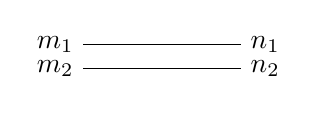
\begin{tikzpicture}{scale=1}
\draw (0,0.3) -- (2,0.3);
\filldraw (0,0.3) circle (0pt) node[left] {$m_1$};
\filldraw (2,0.3) circle (0pt) node[right] {$n_1$};
\draw (0,0) -- (2,0);
\filldraw (0,0) circle (0pt) node[left] {$m_2$};
\filldraw (2,0) circle (0pt) node[right] {$n_2$};
\end{tikzpicture}
\end{center}


\begin{itemize}
\item a ribbon carries 4 bounded indices

\item conservation of the indices along each line

\item characterized by a set of positive integer $(V,I,F,B)$

\begin{itemize}
\item $V$ : number of vertices

\item $I$ : number of internal ribbons

\item $F$ : number of faces

\item $B$ : number of boundaries, equal to the number of closed lines with external legs

\end{itemize}

\item $\mathcal{L}$ : number of ribbon loops, given by

\begin{equation*}
\mathcal{L}=F-B
\end{equation*}

\item $g\in\mathbb{N}$ : genus of the Riemann surface on which $\mathcal{D}$ can be drawn

\begin{equation*}
2-2g=V-I+F 
\end{equation*}


\end{itemize}

\end{frame}

%----------------------------------------------------------------------------%

\begin{frame}

\frametitle{Finiteness -- ``Truncated model'' III}

\textbf{Amplitude} ${\mathbb{A}}^{\cal{D}}$ for a general ribbon diagram :

\begin{itemize}
\item $V$ vertex factors\\
$\to$ \ each vertex contributing to $w(j)$

\item $I$ propagators \\
$\to$ \ each propagator contribute to
%
\begin{equation*}
G^{-1} \ \sim \ \frac{\Pi(M,j)}{w(j)} 
\end{equation*}


\item summations over indices corresponding to $F-B$ loops which give an overall factor bounded by 

\begin{equation*}
(2j+1)^{2(F-B)} 
\end{equation*}

\end{itemize}

\begin{equation*}
{\mathbb{A}}^{\cal{D}}\le Kw(j)^{V-I}\Pi(M,j)^{I}(2j+1)^{2(F-B)}=K^\prime\frac{w(j)^{V-I}(2j+1)^{2(F-B)}}{(j^2+\rho^2)^I}
\end{equation*}

where 

\begin{itemize}
\item $K$ and $K^\prime$ are finite constants and $\rho^2=\frac{M}{\lambda\mu^2}$

\item $w(j)=j+1$ 

\end{itemize}

\end{frame}
%----------------------------------------------------------------------------%

\begin{frame}

\frametitle{Finiteness -- ``Truncated model'' IV}

\begin{exampleblock}{}
\vspace*{-3pt}
\begin{equation*}
{\mathbb{A}}^{\cal{D}} \leq K^\prime\frac{w(j)^{V-I}(2j+1)^{2(F-B)}}{(j^2+\rho^2)^I}
\end{equation*}
\end{exampleblock}

It is a (positive) function of $j$, finite and non singular for $j=0$ 

\begin{equation*}
\mbox{we set} \quad w(j)\sim j, \quad \mbox{for} \ j\to\infty
\end{equation*}

Thus we have the condition

\begin{equation*}
\omega(\mathcal{D})=I+2B+2(2g-2)+V\ge0
\end{equation*}

\begin{itemize}

\item For $g\ge1$, one has $\omega(\mathcal{D})>0$. 

\item For $g=0$

\begin{equation*}
\omega(\mathcal{D})= I+2B+V-4\ge0 
\end{equation*}

\begin{itemize}
\item $V\geq2$ : $\omega(\mathcal{D})>0$ 

\item $V=1$ : 2-point function for the truncated model $\to$ finite

\end{itemize}

\end{itemize}

\begin{block}{}
\vspace*{-14pt}
\begin{center}
the truncated model is finite to all orders in perturbation. 
\end{center}
\vspace*{-9pt}
\end{block}


\end{frame}

%----------------------------------------------------------------------------%

\begin{frame}

\frametitle{Finiteness to all orders I}

\textbf{Back to our gauge model}

\begin{itemize}
\item differs from the truncated model only through the propagator

\begin{equation*}
P^{j_1j_2}_{mn;kl} = \frac{g^2}{8\pi\lambda^3} \frac{1}{w(j_1)\left(M+\lambda^2\mu j_1(j_1+1)+
\tikz[baseline]{\node[fill=black!28!white,anchor=base] (t1) {$\frac{4}{\lambda^2}(k^2+l^2)$};}
\right)}\delta^{j_1j_2}\delta_{ml}\delta_{nk}
\end{equation*}

\item generic structure of $\mathfrak{A}^j_{\mathcal{D}}$
%
\begin{equation*}
\mathfrak{A}^j_{\mathcal{D}} = \sum_{\mathcal{I}} \prod_\lambda P^j_{m_\lambda(\mathcal{I}) n_\lambda(\mathcal{I});k_\lambda(\mathcal{I}) l_\lambda(\mathcal{I})} \ F^j(\delta)_{m_\lambda(\mathcal{I}) n_\lambda(\mathcal{I});k_\lambda(\mathcal{I}) l_\lambda(\mathcal{I})}
\end{equation*}

where 

\begin{itemize}
\item $\mathcal{I}$ : set of (internal) indices $\subset$ $\{-j,...j\}$ so that all sums $\sum_{{\cal{I}}}$ are finite

\item $\lambda$ : labels the internal lines of ${\cal{D}}$

\item $P^j_{mn;kl}$ : (positive) propagator

\item $F^j(\delta)_{mn;kl}$ collects all the delta's plus vertex weights depending only on $j$
\end{itemize}

\end{itemize}

\end{frame}

%----------------------------------------------------------------------------%

\begin{frame}

\begin{itemize}

\frametitle{Finiteness to all orders II}

\item One has the following estimate
%
\begin{eqnarray*}
\vert\mathfrak{A}^j_{\mathcal{D}}\vert &\le& \sum_{\mathcal{I}} \prod_\lambda \left|(G^{-1})^j_{m_\lambda(\mathcal{I}) n_\lambda(\mathcal{I}) ; k_\lambda(\mathcal{I}) l_\lambda(\mathcal{I})} \right| \ \left| F^j(\delta)_{m_\lambda({\cal{I}}) n_\lambda({\cal{I}});k_\lambda({\cal{I}}) l_\lambda({\cal{I}})} \right|
\end{eqnarray*}

\item From the previous condition

\begin{equation*}
\omega(\mathcal{D})=\alpha I+2B+V(2-\alpha)-4\ge0 
\end{equation*}

we have

\begin{equation*}
\vert\mathfrak{A}^j_{\mathcal{D}}\vert \le K^\prime\frac{w(j)^{V-I}(2j+1)^{2(F-B)}}{(j^2+\rho^2)^I}< \infty
\end{equation*}

\end{itemize}

\begin{block}{Finiteness to all orders}
All ribbon amplitudes in our gauge theory $\left(\Omega=1\right)$ are finite so that $S^f_{\Omega=1}$ is perturbatively finite to all orders. $\leadsto$ generalized to $\Omega \neq 1$
\end{block}

\begin{enumerate}
 \item a sufficient rapid decay of the propagator at large indices (large $j$) so that correlations at large separation indices disappear
\item the special role played by $j$, the radius of the fuzzy sphere components act as a cut-off
\item the existence of an upper bound for the propagator that depends only of the cut-off
\end{enumerate}

\end{frame}

%----------------------------------------------------------------------------%

\begin{frame}

\frametitle{Solvability}

We rewrite the action

\begin{equation*}
S^f_\Omega = \frac{2}{g^2} \mbox{Tr}\left( \Phi Q \Phi^\dag + \Phi^\dag Q\Phi \right) + \frac{16}{g^2} \mbox{Tr}\left( (\Omega+1) \Phi\Phi^\dag\Phi\Phi^\dag + (3\Omega-1) \Phi\Phi\Phi^\dag\Phi^\dag \right)
\end{equation*}
 
with the complex fields
%
\begin{equation*}
\Phi=\frac{1}{2}(\Phi_1+i\Phi_2) \qquad \Phi^\dag=\frac{1}{2}(\Phi_1-i\Phi_2)
\end{equation*}
$\bullet$ \ \textbf{Particular case :} $\Omega=1/3$ \quad (Nucl.Phys.B 2016, \ \texttt{[arxiv:1603.05045]})

\begin{itemize}
\item Kinetic operator :
%
\begin{equation*}
Q = K - \frac{8i}{3} L(\theta_3) D_3
\end{equation*}


\item Interaction term : 
%
\begin{equation*}
S_4 = \frac{64}{3g^2} \mbox{Tr}\left( \Phi\Phi^\dag\Phi\Phi^\dag\right)
\end{equation*}
$\to$ \ depends only on $\Phi\Phi^\dag$

\item action is formally similar to the action describing an exactly solvable LSZ-type model

\item partition function for $S^f_{\Omega=\frac{1}{3}}$ can be related to $\tau$-functions of integrable hierarchies

\end{itemize}


\end{frame}

%----------------------------------------------------------------------------%

%\begin{frame}

%\frametitle{Solvability II}

%The partition function can be factorized as
%
%\begin{equation*}
%Z(Q) =\prod_{j\in\frac{\mathbb{N}}{2}} Z_j(Q)
%\end{equation*}

%with

%\begin{equation*}
%Z_j(Q) =\int{\mathcal{D}} \Phi^j \mathcal{D} \ \Phi^{\dag j} \ \text{exp}\left(-\frac{w(j)}{g^2}\mbox{tr}_j \left( 2 \left(\Phi^j Q^j\Phi^{\dag j}+\Phi^{\dag j} Q^j\Phi^j\right)+\frac{64}{3}\left(\Phi^j\Phi^{\dag j}\Phi^j\Phi^{\dag j}\right) \right)\right)
%\end{equation*}

%where

%\begin{equation*}
%\mathcal{D} \Phi^j \ \mathcal{D} \Phi^{\dag j} := \prod_{-j\le m,n\le j} \mathcal{D} %\Phi^j_{mn} \mathcal{D} \Phi^{\dag j}_{mn}
%\end{equation*}

%The Harish-Chandra/Itzykson-Zuber measure formula gives :

%\begin{equation*}
%Z_j(Q) \sim \frac{1}{\Delta^2(Q^j)} \ \det_{-j\le m,n\le j} %\left(f(\omega^j_m+\omega^j_n)\right)
%\end{equation*}

%$\Delta(Q^j)$ : Vandermonde determinant associated with the matrix $Q^j$\\
%$\omega^j_k$ are the eigenvalues of the real symmetric matrix defined by the propagator\\
%$f(z)$ : some known function 

%\end{frame}

%----------------------------------------------------------------------------%

\begin{frame}[plain]

\vspace*{88pt}

\begin{flushright}
\LARGE{\texttt{Thank you.}}
\end{flushright}

\end{frame}

%============================================================================%
\end{document} 
%============================================================================%